\section{ Blockchain }
 Blockchain  o en español cadenas de bloques es una base de datos que puede ser utilizada de forma compartida 
con  usuarios que interactúan entre ellos de la manera peer-to-peer. La  Blockchain   almacena información y 
brinda la característica de inmutar los datos y estructurarlos ordenadamente \cite[]{retamal_Blockchain_2017}.

En ocasiones se confunde esta tecnología con el Bitcoin, pero el Bitcoin es una moneda digital que utiliza la   Blockchain  y está 
programada de una forma para obtener un mayor grado de  seguridad y pseudo anonimato en comparación a otras  Blockchain  
\cite[]{choo_Blockchain_2020}.

En el caso del Bitcoin los datos son públicos y pueden ser consultados en cualquier momento por cualquier 
usuario. 
Entonces la  Blockchain  es una base de datos compartida y descentralizada donde la modificación de las 
transacciones sea casi imposible \cite[]{retamal_Blockchain_2017} , los datos (registros o transacciones) son 
almacenados dentro de un bloque y puede contener una o más transacciones, para que los bloques sean agregados a la   Blockchain . 
La mayoría de los nodos deben estar de acuerdo mediante algún tipo consenso o protocolo para validar la integridad de los bloques\cite[]{choo_Blockchain_2020} \cite[]{retamal_Blockchain_2017}.

Los nodos deben ejecutar algún tipo de consenso o protocolo para obtener un acuerdo  de que transacciones se 
almacenan en la  Blockchain  para esto existen diferentes consensos, como la \gls{pow} \cite[]{retamal_Blockchain_2017} ,\gls{pos} \cite[]{drescher_Blockchain_2017}, 
\gls{poa}, depende del algoritmo utilizado se requiere más o menos recursos y se obtiene 
más o menos seguridad \cite[]{retamal_Blockchain_2017}. 
Estas bases de datos compartidas permiten que los registros almacenados no sean alterados. Para identificar 
quien es el propietario de los datos almacenados se le asigna una clave pública (identificadores visibles por
todos los nodos de la red) y una clave privada al usuario (utilizado para firmar las transacciones) 
\cite[]{retamal_Blockchain_2017}.
\subsection{Funcionamiento de la Blockchain}
 La  Blockchain como se ha descrito anteriormente, es una base de datos compartida
 por todos los usuarios de una red peer to peer, el caso de las  Blockchain publicas esos datos
 pueden ser accedido en cualquier momento y por cualquier usuario. 
 La información añadida a la cadena de bloques pasa por un protocolo de consenso,
 o proceso para confirmar que la información que se pretende almacenar es correcta y cumple
 con las reglas definidas en la red.

Los nodos de la  Blockchain son pares iguales, en cada nodo se contiene la misma información con todas las transacciones realizadas
dentro de un bloque, cada bloque contiene un numero de transacciones, en el caso de Bitcoin contiene alrededor de unas dos mil transacciones aproximadamente.
\cite[]{retamal_Blockchain_2017}

Las llamadas transacciones, son los mensaje que se envían de una dirección a otra, en ella 
 se almacenan datos, como cantidades de una cierta moneda a gastar o datos alfanuméricos, estos datos dependen 
 como se haya definido las reglas de Blockchain. Pero por lo generar las transacciones transmiten una cantidad de una criptomoneda y adjuntan 
 datos extras. Ellas son enviadas a todos los nodos de la red en donde existe una competencia por quien de los  nodos va almacenar primero el bloque con la 
 mayoría de las transacciones nuevas dentro de un bloque. La competencia se debe a que el nodo que resuelva un problema para poder agregar el bloque 
 recibe una recompensa con la criptomoneda nativa de su  Blockchain  como en el caso de la prueba de trabajo, lo cual los nodos compiten
 por quien obtiene un hash el cual identificara al bloque  con ciertas reglas como ser iniciar el hash con una cantidad de ceros, de esta manera trabaja 
 Bitcoin, existen también otros tipos de competencias ellas son denominadas algoritmos de consensos o protocolos de consensos.
Esto sirve para incentivar a los usuarios ser parte de la red, ya que pueden obtener recompensas, a mayor cantidad de nodos, la red se vuelve mas segura.

El bloque nuevo se agrega a la base de datos apuntando al hash que representa el bloque anterior, de esta manera
cada bloque “ apunta ” hacia el bloque que le precede  pudiendo ir hasta la raiz y obtener todo el historial de las transacciones.
Los bloques almacenan información extras como el tiempo en el cual el bloque fue agregado a la cadena, la referencia hacia el bloque anterior, y otros 
datos dependiendo de las reglas que se han programado.
En la figura \ref{img:nakamoto_bloque} de la  página \pageref{img:nakamoto_bloque} muestra la estructura de un bloque, donde lo TX representan 
las transacciones almacenadas en el bloque y el nonce es el numero que hace que hash del bloque cumpla con las reglas definidas para 
la competencia, por ejemplo si se necesita que el hash del bloque inicie con tres ceros, los competidores prueban diferentes valores, en el nonce
hasta hallar el hash que inicie con los tres ceros, esto no ocurre en todas las Blockchain, sino en las que cuentan con
el algoritmo de consenso prueba de trabajo. \cite[]{nakamoto_bitcoin_2008,drescher_Blockchain_2017,kelly_investigation_2018,ethereum_org_transactions_2021}

\begin{figure}[hbt!]
    \centering
    {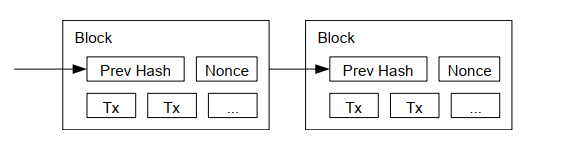
\includegraphics[scale=1]{nakamoto_bloque.png}}
    \caption{Estructura de una cadena de bloque genérica \cite[]{nakamoto_bitcoin_2008}}
    \label{img:nakamoto_bloque}
\end{figure}


La criptomoneda de la  Blockchain es definida como una cadena de firmas digitales, donde cada dueño transfiere la moneda al próximo,
firmando digitalmente el hash de la transacción previa y la clave publica del destinatario. entonces en la transacción se almacena el hash
mas el hash pero con la firma del emisor de la transacción, con lo cual se puede comprobar quien fue el emisor y también quien es el receptor.
Esta explicación se puede observar gráficamente en la figura \ref{img:nakamoto_transaccion} de la  página \pageref{img:nakamoto_transaccion}
\cite[]{nakamoto_bitcoin_2008}

\begin{figure}[hbt!]
    \centering
    {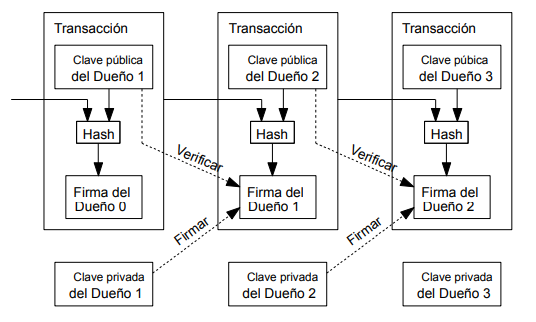
\includegraphics[scale=1]{nakamoto_transaccion.png}}
    \caption{Figura de una transacción \cite[]{nakamoto_bitcoin_2008}}
    \label{img:nakamoto_transaccion}
\end{figure}

Con este protocolo cuando mas grande es la red, es mas difícil poder modificar sus estados actuales, 
porque un nodo que modifique algún estado interno ya almacenado,
tiene que ser verificados para que todos los nodos los agreguen, si ven que no cumple con las reglas, o los datos
no son los mismos que los demás nodos, se rechaza. 
Por ende los datos almacenados en la BLockchain no pueden ser modificados, sin que todos los nodos lo modifiquen.
El autor de un ataque malicioso deberá tener el control de la mitad mas un nodo para poder realizar sus acciones, pero esto resulta
muy costoso y a medida que la red crece, cada vez es mas difícil relanzarlo ya que el poder de computo de la red se vuelve mas compleja. \cite[]{joaquin_lopez_lerida_economiBlockchain_2016,nakamoto_bitcoin_2008}

Un minero es un nodo en la red que recopila transacciones y trabaja para organizarlas en bloques, 
ellos cada vez que reciben una transacción verifican si es correcta, y por el trabajo que realizan se les da una recompensa,
que son una pequeña comisión que es cobrada al emisor de la transacción y dependiendo del algoritmo de consenso, también se minan nuevas 
criptomoneda por bloque almacenado. Al mantener incentivados a los mineros se crea una red que incrementa sus nodos por ende mas  segura \cite[]{preukschat_Blockchain_2018,joaquin_lopez_lerida_economiBlockchain_2016,nakamoto_bitcoin_2008}  

\subsection{Características de una Blockchain}

Las características principales de una  Blockchain son:

\begin{itemize}
    \item Seguridad y Privacidad: Los usuarios de la red pueden realizar transacciones libremente sin brindar ningun tipo de información personal
    simplemente firmando con su clave privada para verificar que le corresponde la clave publica. Pero la seguridad de las cadenas de bloques es en la manera que
    se conectan, donde un bloque apunta al anterior y genera un hash nuevo a partir de ella y las transacciones almacenadas, por lo tanto si algún dato del 
    bloque anterior es modificada, el hash del siguiente bloque cambiaría y 
    la cadena almacenada en el nodo no concordaría con los demás nodo, entonces las acciones de este nodo serían rechazadas por las demás, 
    ya que la información no concuerda con los otros.  
    
    \item Trazabilidad: Es posible realizar un rastreo de todas las operaciones que se han realizado con una address especifica, y también conocer 
  los recorridos de las transacciones que se han ejecutado , ya que todas ellas se encuentran enlazadas y 
    almacenadas en los nodos de la Blockchain. 

    \item Transparencia: Se logra publicando las reglas que definen el funcionamiento de la  Blockchain y haciendo publico el código fuente
    del software, cualquier individuo puede acceder al funcionamiento del software, por lo tanto es conocible el comportamiento del software.
    \item Confianza: No es necesaria la confianza entre dos usuarios para realizar una transacción ya que el protocolo se encarga de realizar 
    el proceso.
    
    \end{itemize}

\subsection{Clases de Blockchain}
Existen las  Blockchain privadas , publicas e híbridas , las publicas son las nombradas a lo largo del documento y son las  Blockchain de Ethereum, EOS, Bitcoin 
. Las primeras  Blockchain fueron diseñadas para ser publicas, cualquier individuo puede acceder sin ser usuario y leer las transacciones, cualquier 
persona o maquina puede convertirse en usuario y participar del protocolo, son descentralizadas todos los nodos son iguales, y pseudoanonimas 
porque los dueños de las transacciones no necesitan brindar ningun dato, por lo cual se desconoce, quien es dueño de una dirección pero si son
rastreable dado su carácter publico. \cite[]{preukschat_Blockchain_2018}

Las  Blockchains privadas tambien denominadas redes de permisos se caracterizan porque  pueden ser accedida y utilizada en algunas o todas las transacciones
por participantes de la red.  También por lo general cuentan con  distintos niveles de accesos según como se halla definido la red, por ejemplo establecer 
diferentes tipos de roles.
Las redes privada están compuesta en la mayoría de los casos de un numero bajo de nodos, ya que la cantidad de participantes 
es limitada, pero la seguridad de la  Blockchain se caracteriza  a mayor números de nodos mayor seguridad. \cite[]{torres_Blockchain_nodate}

Combinando las características de las Blockchains públicas y privadas nos encontramos las
Blockchains híbridas. La  diferencia con las publicas y privadas  es 
en el protocolo de consenso. En lugar de ser un sistema abierto donde todos pueden validar los
bloques o uno cerrado donde una única entidad ejerce todo el control, nos encontramos con una
red donde el proceso de consenso es controlado por varias entidades, un grupo de nodos
funcionan como validadores de las transacciones.\cite[]{torres_Blockchain_nodate}




%% cambiar lo de abajo y modificar antes estaba en antecedentes
